\chapter{Prezentare turbine "AXENT"}\label{chapter:prezentare}


\section{Utilitate si utilizare}

\^{I}n ultimii ani, \^{i}n cadrul Institutului de ma\c{s}ini hidraulice din Universitatea Stuttgart, a avut loc cercetarea posibilit\u{a}\c{t}ilor de recuperare a energiei hidraulice \^{i}n anumite situa\c{t}ii speciale din industrie. Astfel a ap\u{a}rut conceptul unei turbine modulare de destindere pentru recuperarea de energie. "Eine modulare axiale Entspannungsturbine" pe scurt AXENT, care este \c{s}i numele comercial al acestei ma\c{s}ini, este rezultatul acestor studii.

Condi\c{t}iile tehnice asumate ini\c{t}ial au presupus g\u{a}sirea de solu\c{t}ii unde avem:

\begin{itemize}
	\item fluid de lucru la presiune ridicat\u{a}
		\begin{itemize}
			\item transport
			\item procese industriale
		\end{itemize}
	\item destinderea presiunii p\^{a}n\u{a} la nivelul dorit
		\begin{itemize}
			\item facut\u{a} prin robine\c{t}i, supape sau arm\u{a}turi
			\item energia poten\c{t}ial\u{a} a presiunii r\u{a}m\^{a}n\^{a}nd nefolosit\u{a}
		\end{itemize}
	\item cre\c{s}terea randamentului prin rec\^{a}\c{s}tigarea de energie
		\begin{itemize}
			\item transformarea energiei hidraulice \^{i}n energie electric\u{a}
			\item far\u{a} a afecta instala\c{t}ia sau procesul deja existent
		\end{itemize}	
\end{itemize}

Pentru situa\c{t}iile enumerate mai sus dorin\c{t}a a fost de a \^{i}ndeplini mai multe lucruri dintre care le voi enumera pe cele mai importante:

\begin{itemize}
	\item proprieta\c{t}i tehnice
		\begin{itemize}
			\item utilizare la debit constant
			\item lipsa \c{s}ocurilor
			\item domeniu de utilizare larg
		\end{itemize}
	\item domenii poten\c{t}iale de utilizare
		\begin{itemize}
			\item alimentare cu ap\u{a}
			\item procese industriale
			\item industria chimic\u{a}
		\end{itemize}
	\item din punct de vedere economic
		\begin{itemize}
			\item recuperare de energie
			\item costuri de realizare \c{s}i intre\c{t}inere c\^{a}t mai mici
		\end{itemize}
	\item obiective politice
		\begin{itemize}
			\item eficientizare ca dorin\c{t}a constant\u{a}
			\item \^{i}mbun\u{a}t\u{a}\c{t}irea bilan\c{t}urilor ecologice
		\end{itemize}	
\end{itemize}

Dup\u{a} analiza tuturor criteriilor pentru care se caut\u{a} o solu\c{t}ie, respect\^{a}nd bine\^{i}n\c{t}eles \c{s}i condi\c{t}iile economice \c{s}i politice, concluzia a fost c\u{a} cel mai bun loc pentru aceast\u{a} viitoare turbin\u{a} este \^{i}n domeniul \textbf{aliment\u{a}rii cu ap\u{a} a ora\c{s}elor mari din zone muntoase.}

\begin{figure}[h!]
	\centering
	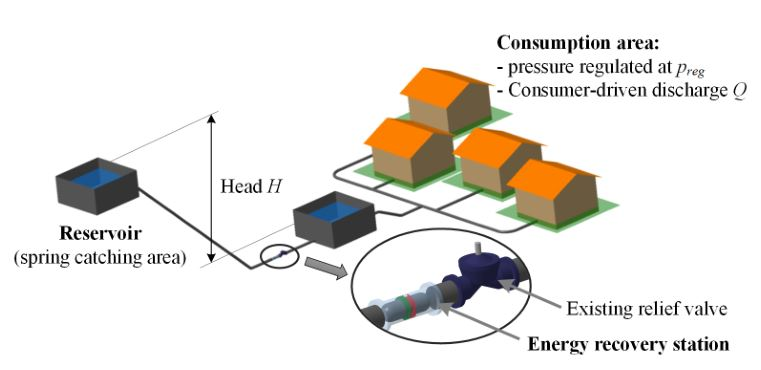
\includegraphics[scale=0.7]{figures/amplasare_turbina.jpg}
	\caption{Amplasare turbin\u{a} \cite{andolfatto2016simulation}}
	\label{Amplasare turbin\u{a}}
\end{figure}

Condi\c{t}iile minime care trebuie \^{i}ndeplinite sunt legate de topografia regiunii, pentru a avea o c\u{a}dere \c{s}i o presiune mare, dar \c{s}i m\u{a}rimea re\c{t}elei de alimentare pentru a asigura debitul necesar func\c{t}ion\u{a}rii turbinei la randament ridicat. \^{I}n principiu este necesar\u{a} o topografie deluroas\u{a} \c{s}i alimentarea cu ap\u{a} s\u{a} se fac\u{a} pentru o comunitate de minim 3000 de locuitori.


\section{Particularitati constructive}

Turbinele de destindere au ca elemente principale un rotor, c\u{a}ruia datorit\u{a} mi\c{s}c\u{a}rii apei \^{i}i este imprimat\u{a} o mi\c{s}care de rota\c{t}ie \c{s}i un generator pentru transformarea lucrului mecanic \^{i}n energie electric\u{a}. Un punct dup\u{a} care putem categorisi turbinele axiale de destindere este pozi\c{t}ia generatorului, varianta "Inline" (vezi Figura 6) cu generator imersat \^{i}n conduct\u{a} imediat dup\u{a} rotor sau cu generator aflat \^{i}n afara conductei de trecere a apei, generator exterior (Figura 1.3).

\begin{figure}[h!]
	\centering
	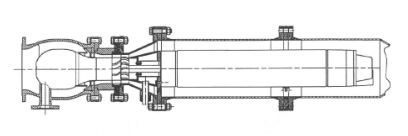
\includegraphics[scale=1.25]{figures/generator_inline.jpg}
	\caption{Generator imersat "Inline" \cite{GREES_2014}}
	\label{Generator imersat Inline}
\end{figure}

\begin{figure}[h!]
	\centering
	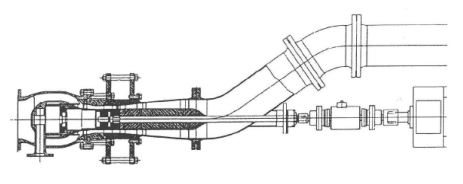
\includegraphics[scale=1.25]{figures/generator_in_afara_conductei.jpg}
	\caption{Generator \^{i}n afara conductei \cite{GREES_2014}}
	\label{Generator \^{i}n afara conductei}
\end{figure}

Dup\u{a} cum se vede \c{s}i \^{i}n ultimele imagini, avantajul turbinei cu generator "Inline" const\u{a} \^{i}n capacitatea de instalare modular\u{a} mult mai simpl\u{a}, prin sec\c{t}ionarea conductei \c{s}i prinderea modulului turbinei prin flan\c{s}e \^{i}n conduct\u{a}.

\begin{figure}[h!]
	\centering
	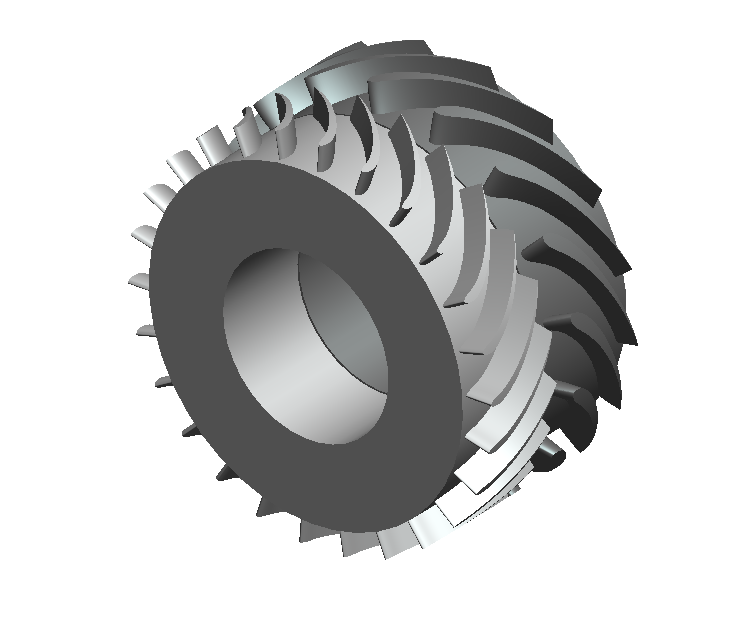
\includegraphics[scale=0.6]{figures/modul_singular.png}
	\caption{Modul singular \cite{susanhub}}
	\label{Modul singular}
\end{figure}

\^{I}n proiectarea modern\u{a} a turbinelor axiale, se folose\c{s}te frecvent teoria hidraodinamic\u{a} a re\c{t}elelor de profile. Metodele numerice de determinare a re\c{t}elelor de profile, care exprim\u{a} legatur\u{a} \^{i}ntre parametrii geometrici \c{s}i cei hidrodinamici au fost folosite \^{i}n cadrul Universit\u{a}\c{t}ii Suttgart pentru a ajunge la un produs cu aplicabilitate imediat\u{a} \c{s}i tangibil\u{a}. Rezultatele acestor cercet\u{a}ri au fost dezvoltarea unei turbine cu aparat director format din 26 profile \c{s}i un rotor cu 30 palete, care se poate folosi \^{i}n modul singular sau \^{i}n dou\u{a} trepte (vezi Figura 1.4 \c{s}i Figura 1.5).

\begin{figure}[h!]
	\centering
	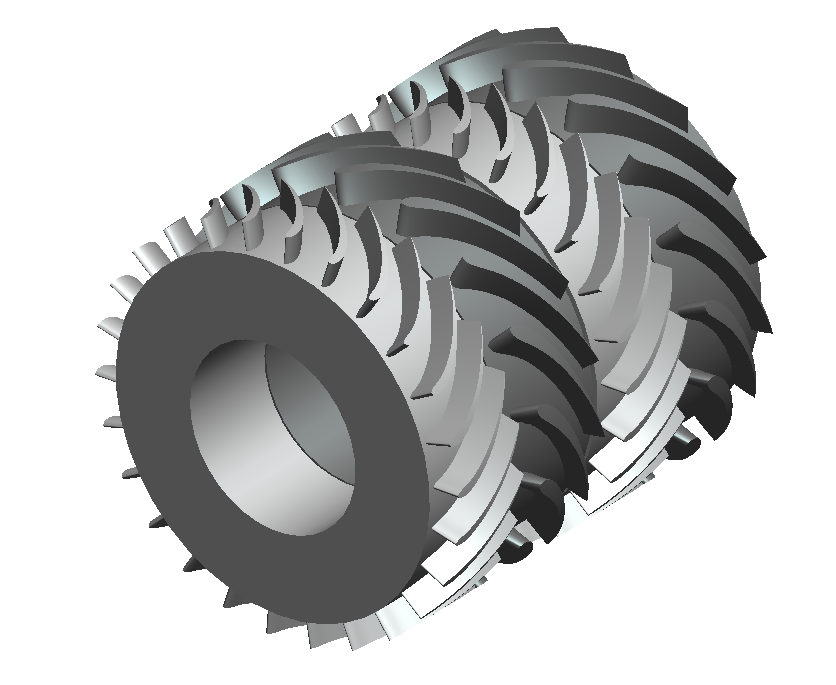
\includegraphics[scale=0.6]{figures/modul_in_doua_trepte.png}
	\caption{Modul \^{i}n dou\u{a} trepte \cite{susanhub}}
	\label{Modul \^{i}n dou\u{a} trepte}
\end{figure}



\subsection{Alte solu\c{t}ii. Turbin\u{a} axial\u{a} cu rotoare contrarotative}

Conceptul de micro turbin\u{a} contrarotativ\u{a} prezentat \^{i}n Figura 10 \c{s}i descris \^{i}n detaliu \^{i}n lucr\u{a}rile \cite{andolfatto2016simulation} \c{s}i \cite{andolfatto2015mixed} este un candidat pentru recuperarea energiei din re\c{t}elele cu ap\u{a} potabil\u{a}, chiar \c{s}i \^{i}n locurile cu putere disponibil\u{a} \^{i}ntre 5 kW \c{s}i 25 kW. Prezint\u{a} o arhitectur\u{a} axial\u{a} compact\u{a} asigur\^{a}nd posibilitatea instal\u{a}rii in-line \^{i}n re\c{t}elele deja existente, limit\^{a}nd astfel cheltuielile financiare \c{s}i impactul asupra mediului \c{s}i infrastructurii.

Aceste ma\c{s}ini opereaz\u{a} la viteze variabile \c{s}i acoper\u{a} o arie ridicat\u{a} de operabilitate. Folosind o vitez\u{a} variabil\u{a} \^{i}ntre cele dou\u{a} rotoare ridic\u{a} de asemenea eficien\c{t}a total\u{a} a turbinei, ridic\^{a}nd astfel veniturile a\c{s}teptate.

\begin{figure}[h!]
	\centering
	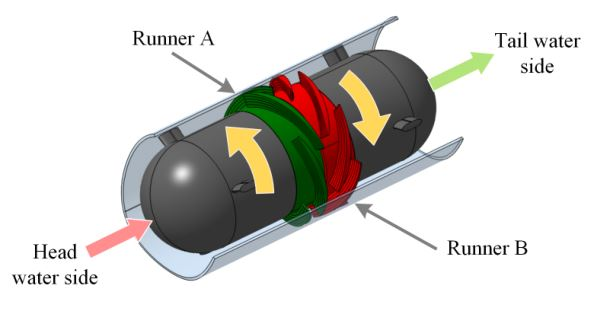
\includegraphics[scale=0.75]{counter_rotating_runners}
	\caption{Turbina contrarotativ\u{a} \cite{andolfatto2016simulation}}
	\label{Turbina contrarotativ\u{a}}
\end{figure}

\clearpage


\subsection{Utilizarea modular\u{a}}
Unul din marile avantaje al acestor turbine axiale de destindere este posibilitatea de a le folosi \^{i}n serie, forma lor compact\u{a} \c{s}i cotele de gabarit reduse \^{i}ncuraj\^{a}nd acest lucru.

\begin{figure}[h!]
	\centering
	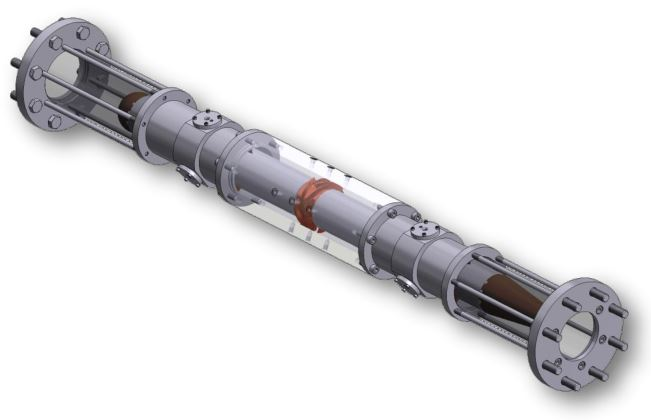
\includegraphics[scale=0.9]{modular}
	\caption{Modular \cite{hasmatuchi2014new}}
	\label{Modular}
\end{figure}

\subsection{Descrierea elementelor componente}

Principalele elemente componente ale turbinei axiale de destindere sunt:

\begin{itemize}
	\item \textbf{statorul}; conduce apa spre rotor \c{s}i asigur\u{a} vitezele respectiv circula\c{t}ia necesar\u{a} transform\u{a}rii energetice optime, \^{i}n condi\c{t}iile pierderilor hidraulice minime.
	\item \textbf{rotorul}; are rolul de a transforma energia hidraulic\u{a} disponibil\u{a} \^{i}n energie cinetic\u{a}, conduc\^{a}nd apa care vine prin stator \^{i}n tubul de aspira\c{t}ie al turbinei.
	\item \textbf{generatorul electric}; este un dispozitiv care transform\u{a} energia mecanic\u{a} \^{i}n energie electric\u{a}.
\end{itemize}


\section{Regimuri de functionare}

Turbinele hidraulice se pot caracteriza din punct de vedere func\c{t}ional prin folosirea urm\u{a}torilor parametri:

\begin{itemize}
	\item debitul \textit{Q, $[\si{m}]$}
	\item c\u{a}derea \textit{H, $[\si{m}]$}
	\item puterea \textit{$P_m$, $[\si{W}]$}
	\item viteza unghiular\u{a} \textit{\(\omega\), $[\si{rad/s}]$}
	\item randamentul \textit{\(\eta\), $[-]$}
	\item \^{i}n\u{a}l\c{t}imea geometric\u{a} de aspira\c{t}ie \textit{\(h_s\), $[\si{m}]$}
	\item coeficientul de cavita\c{t}ie \textit{\(\sigma\), $[-]$}
\end{itemize}


\subsubsection{Debitul}

Definim debitul volumic ca volumul de ap\u{a} ce intr\u{a} \^{i}n turbin\u{a} \^{i}n unitatea de timp. Se exprim\u{a} \^{i}n unit\u{a}\c{t}i de volum, greutate sau de mas\u{a}, raportate la unitatea de timp.


\subsubsection{C\u{a}derea turbinei}

Consider\^{a}nd sec\c{t}iunea de la intrarea \^{i}n turbin\u{a} ca notat\u{a} cu i \c{s}i ie\c{s}irea cu e, c\u{a}derea turbinei se exprim\u{a} sub forma $H=e_i-e_e$, deci

\begin{equation}
H=\bigg(\frac{p_i}{{\rho}g}+z_i+\frac{v_i^2}{2g}\bigg)_i-\bigg(\frac{p_e}{{\rho}g}+z_e+\frac{v_e^2}{2g}\bigg)_e \;[\si{m}]
\end{equation}

unde: $p\;[\si{Pa}]$ este presiunea, ${\rho}\;[\si{kg/m^3}]$ este densitatea apei, $z\;[\si{m}]$ este \^{i}n\u{a}l\c{t}imea, $v\;[\si{m/s}]$ este viteza iar $g\;[\si{m/s^2}]$ este accelera\c{t}ia gravita\c{t}ional\u{a}.

\subsubsection{Puterea}

Puterea hidraulic\u{a} sau puterea sursei $P_h$ este puterea disponibil\u{a} a apei de la intrarea \^{i}n turbin\u{a} pentru a putea fi transformat\u{a} \^{i}n putere mecanic\u{a} la arborele turbinei:

\begin{equation}
P_h={\rho}gQH\; [\si{W}]
\end{equation}

Puterea mecanic\u{a} a turbinei $P_m$ este puterea mecanic\u{a} la arborele turbinei, ob\c{t}inut\u{a} din momentul la arbore $M$ \c{s}i viteza unghiular\u{a} $\omega$:

\begin{equation}
P_m=M{\omega}\; [\si{W}]
\end{equation}

\subsubsection{Tura\c{t}ia}

Rota\c{t}ia sau tura\c{t}ia turbinei este num\u{a}rul de \^{i}nv\^{a}rtituri realizate \^{i}n unitatea de timp, de obicei \^{i}ntr-un minut (uneori \^{i}n secund\u{a}). Se noteaz\u{a} cu \textit{n} [rpm] sau cu \(\omega\) rad/s (SI).

\begin{equation}
n\; [\si{rpm}]\rightarrow{\omega}\; [\si{rad/s}]=\frac{{\pi}n}{30}
\end{equation}


\subsubsection{Randamentul}

\^{I}n turbina hidraulic\u{a} transmiterea energiei de la curentul de ap\u{a} c\u{a}tre rotor se efectueaz\u{a} cu pierderi. Aceastea sunt definite \c{s}i m\u{a}surate prin randamentul turbinei:

\begin{equation}
{\eta}=\frac{Putere\; utila}{Putere\; consumata}=\frac{P_m}{P_h}=\frac{M{\omega}}{{\rho}gQH}
\end{equation}


\subsubsection{In\u{a}ltimea geometric\u{a} de aspiratie}

\^{I}n\u{a}l\c{t}imea geometric\u{a} de aspira\c{t}ie este diferen\c{t}a \^{i}n plan vertical dintre o referin\c{t}\u{a} a turbinei (de obicei planul care trece prin axa paletelor rotorului) \c{s}i planul nivelului apei din aval.

\subsubsection{Coeficientul de cavita\c{t}ie}

Cavita\c{t}ia este un fenomen hidrodinamic complex, caracterizat de apari\c{t}ia, dezvoltarea \c{s}i surparea rapid\u{a} a unor bule cavita\c{t}ionale, umplute cu aburi \c{s}i gaze, ce apare \^{i}ntr-un curent de lichid \^{i}n zona cu viteze mari \c{s}i presiuni mici. Procesul fizic numit cavita\c{t}ie se apropie mai mult sau mai pu\c{t}in de acela al fierberii lichidelor. Efectele principale ale cavita\c{t}iei sunt: vibra\c{t}ii \c{s}i zgomote puternice, distrugerea materialului componentelor turbinei \c{s}i scaderea randamentului de func\c{t}ionare.

Aceste fenomene se intensifica atunci când pragul de cavitație limita este depășit, sau se funcționează în supercavitatie. Profesorul D.Thoma a introdus pentru prima oara noțiunea de prag de cavitație. Acest criteriu este denumit coeficient de cavitație și se exprima în felul următor:

\begin{equation}
\sigma=\frac{A-A\pm{H_s}}{H}
\end{equation}


\subsection{Valori tipice pentru parametrii fundamentali ai turbinelor de destindere}

In literatura de specialitate sunt investigate turbinele de destindere cu valori fundamentale care se încadrează deseori intre anumite limite.


\subsubsection{Debitul}
Pentru debitul volumetric valorile generale pe care le găsim în articolele științifice sunt următoarele:

\begin{itemize}
	\item 0.2500$\si{m^3/s}$ \cite{gentner2000experimentelle}
	\item 0.1200-0.1900$\si{m^3/s}$ \cite{GREES_2014}
	\item 0.0500-0.1450$\si{m^3/s}$ \cite{susanhub}
	\item 0.0090-0.0140$\si{m^3/s}$ \cite{biner2016engineering}
	\item 0.0375$\si{m^3/s}$ \cite{hasmatuchi2014new}
\end{itemize}


\subsubsection{C\u{a}derea}

\begin{itemize}
	\item 50$\si{m}$ \cite{gentner2000experimentelle}
	\item 40-200$\si{m}$ \cite{GREES_2014}
	\item 10.2-205.4$\si{m}$ \cite{susanhub}
	\item 24.265-61.162$\si{m}$ \cite{biner2016engineering}
	\item 29.9$\si{m}$ \cite{hasmatuchi2014new}
\end{itemize}


\subsubsection{Tura\c{t}ia}

\begin{itemize}
	\item 1500$\si{rpm}$ \cite{gentner2000experimentelle}
	\item 3000$\si{rpm}$ \cite{GREES_2014}
	\item 1500 și 3000$\si{rpm}$ \cite{susanhub}
	\item 3000$\si{rpm}$ \cite{biner2016engineering}
	\item 3000$\si{rpm}$ \cite{hasmatuchi2014new}
\end{itemize}

Bazându-ne pe rezultatele din aceste studii putem concluziona ca domeniile de funcționare din Tabela 1.1 reprezinta un punct de plecare acceptabil pentru studiul care urmează în aceasta lucrare de disertație. Aceste valori ne permit proiectarea unei turbine care respecta condiția inițiala autoimpusa, aceea de a nu influența cu nimic buna desfășurare a procesului de alimentare cu apa, turbina producând energie pe o plaja mare de funcționare, fără defecțiuni și fără nevoia unei intervenții din exterior.\\

\begin{table}[ht]
\caption{Domeniile de funcționare dorite ale turbinei AXENT \cite{neipp2017zweistufige}}% title of Table
\centering

\begin{tabular}{ c | c | c | c | c | c | c }
            & Q_{min}          & Q_{max}          & H_{min}    & H_{max}     & n_{min}        & n_{max} \\ \hline
&&&&&&\\[-0.5em]
Valori țintă  & 0.05$\si{m^3/s}$ & 0.15$\si{m^3/s}$ & 10$\si{m}$ & 180$\si{m}$ & 1500$\si{rpm}$ & 6000$\si{rpm}$ \\
\end{tabular}

\end{table}

\clearpage